\documentclass[14pt, a4paper]{book}

\usepackage{cmap} % поиск в pdf
\usepackage[T2A]{fontenc} % кодировка
\usepackage[utf8]{inputenc} % кодировка исходного кода
%\usepackage[kazakh]{babel}
\usepackage{hyperref}
\usepackage{graphicx}
\graphicspath{./images/}

\renewcommand{\chaptername}{Бөлім} % Chapter-і өзгертеді екен
\author{Дәулет}
\title{Latex тесттен өткізіп жатырмын}
\date{\today}

\begin{document}
    \maketitle

    \tableofcontents{}
    \clearpage

    \chapter{Кіріспе}
    \section{Бірінші бөлім}
    \textbf{Python программалау тілі} - бұл қәзіргі уақытта әлемде ең кең 
    таралған программа тілі болып саналады. Бірінші бөлімде Python 
    программа тіліне кіріспе бөлімі.

    \begin{itemize}
        \item Бірінші
        \item Екінші
        \item үшінші
        \item төртінші
    \end{itemize}

    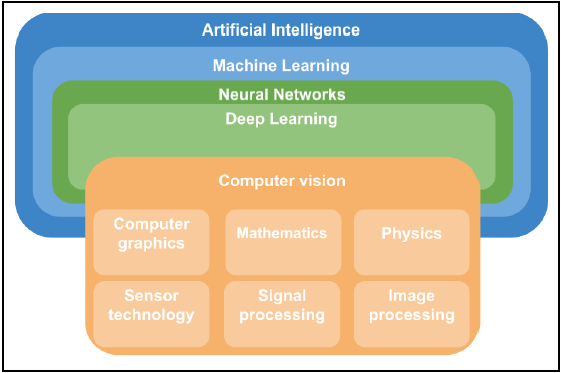
\includegraphics[scale=0.6]{images/cv-1.png}

    Сілтеме \ref{example}
    \section{Екінші бөлім}
    Екінші бөлімде Python программалау тілінің синтаксисіне кіріспе
    бөлім ретінде қарастырамыз.

    \label{example}
    for i in range(10):
        print(i)
\end{document}